<<<<<<< 9e86ad4a1f355e7c69e326775c8b5cbbd729aac8
%-----------------------------------------------------------------------
%\subsection{Introduction}
%-----------------------------------------------------------------------
%\tbc
%

\section{Motivation}
%\tbc
	%BaseliyosJacob
The openETCS work package 3 (WP3) aims to provide – amongst others - the software architecture for the openETCS kernel in order to eventually build the software itself. WP3  partner has put great effort in the openETCS software design, thus far without making definite choices on the software architecture itself respective of functional breakdown and data structures of the openETCS kernel. Since the project planning foresees in the production of a reference software to be used as a demonstrator by June 2015, it is of paramount importance that a first design delivarable of the openETCS kernel architecture be finalized shortly but no later than November 2014.\\

In compliance with the agreements made during the last WP 3 meeting at the 10.09.2014 in Brussels, DB has taken the initiative to design the aforesaid architecture including of functional breakdown and data structures in order to safeguard a timely delivery of these products. Furthermore, DB has ensured that these developments are focused on including end user requirements so as to develop a design in conformity with the needs and requirements of the operators. Specialists of DB and NS have cooperated together with other partners in WP3 to produce this document.\\

As referred to above, the architecture description has to be finalized in the month of November 2014. This version of the document is a draft version, demonstrating the general directions and philosophy of the architectural design, the functional breakdown of the software and the data structures. The design is focused on maximum efficiency in order to maximize on RAMS performance of the end product.\\


\section{Objectives}
%\tbc
%Baseliyos Jacob
The prime objective of WP3 is to produce a fully formal prototype for the openETCS reference system that can function as a demonstrator in collaboration with WP 4 and WP 5  for the openETCS approach and will be used as such in the final phase of the project. That phase is the first half of 2015.  This objective is defined as … 

\textbf{High level Objectives of this work:}
<<any further general statements on the ITEA2  objectives, like…>>\\

\begin{itemize}
\item Work on a model bases approach and process for effective collaborative work within an international ETCS developer team as stated above, the project needs a definite architecture design by the end of 2014.

\textbf{This document targets:}
\item Defining the general design and conditions of the openETCS architecture, functional breakdown and data structures
\item Providing the guidelines for discussion during the workshops that are planned in October and November 2014 that will result in the final and decisive version of this document
\item Being the ‘platform’ for finalization i.e. whatever be the products or results of the workshops shall be integrated in this document.

\textbf{Apart from these general objectives, the document means to provide for the materials that will enable WP3 partners to improve the efficiency of the Work Package activities:}
\item The comprehensive architecture design shall enable splitting the work load according to the building blocks defined by the architecture and allocate strictly compartmented work parcels or activities to WP3 partners.
\item Doing so will enable WP3 to avoid any double work
\item  Compartmenting the work load according to the functional building blocks as defined by the architecture will enable efficient planning of activities, be it individually or the integrated WP3 planning for the coming period, aiming at a just in time delivery of all results and products
\item  Compartment the work load according to the functional building blocks as defined by the architecture will enable efficient planning of activities, be it individually or the integrated WP3 planning for the coming period, aiming at a just in time delivery of all results and products
\end{itemize}

%\tbc
%JakobGärtner


\section{Objectives and scope of deliverables}

The prime original objective of WP3 was to produce a rapid prototype for the openETCS reference system that can function as a demonstrator in collaboration with WP 4 and WP 5  for the openETCS approach and will be used as such in the final phase of the project. That phase is the first half of 2015. \\

We have to see this original objective in the context of the overall innovation promise of openETCS and the related exploitation potential.
Taking into account the current situation of the project (as of Nov. 2014) we have to make choices that make sure that the remaining budget and resources are wisely used, which necessitates that the WP3 deliverables become more "multi- purpose":

 •  provide a functional formal specification of openETCS, based on functional analysis, and traceable to the SRS.
 
 •  Iteratively develop the software architecture and design description document (ADD) while using the formal specification as an executable functional model
 
 •  Utilise real- world use-case scenarios as early as possible in the development process
 
If we take this approach, we can use the iterative development method, while applying a pragmatic view of SCRUM (which has been defined as the high- level project management method for this project) in order to build the following deliverables:

 •  An ADD document, providing a functional description of software architecture and design.
 
 •  A RFC (Request For Comment) process that provides a cross- reference to the SRS, listing all requirements and design conflicts that have been identified during our work
 
 •  A formal, executable model of the openETCS kernel, which can directly be used as entry point into a (future) EN5012x SIL4 compliant software design process, as well as functional reference during simulation and on the planned WP5 demonstrator.
 
 
\begin{figure}
  \centering
  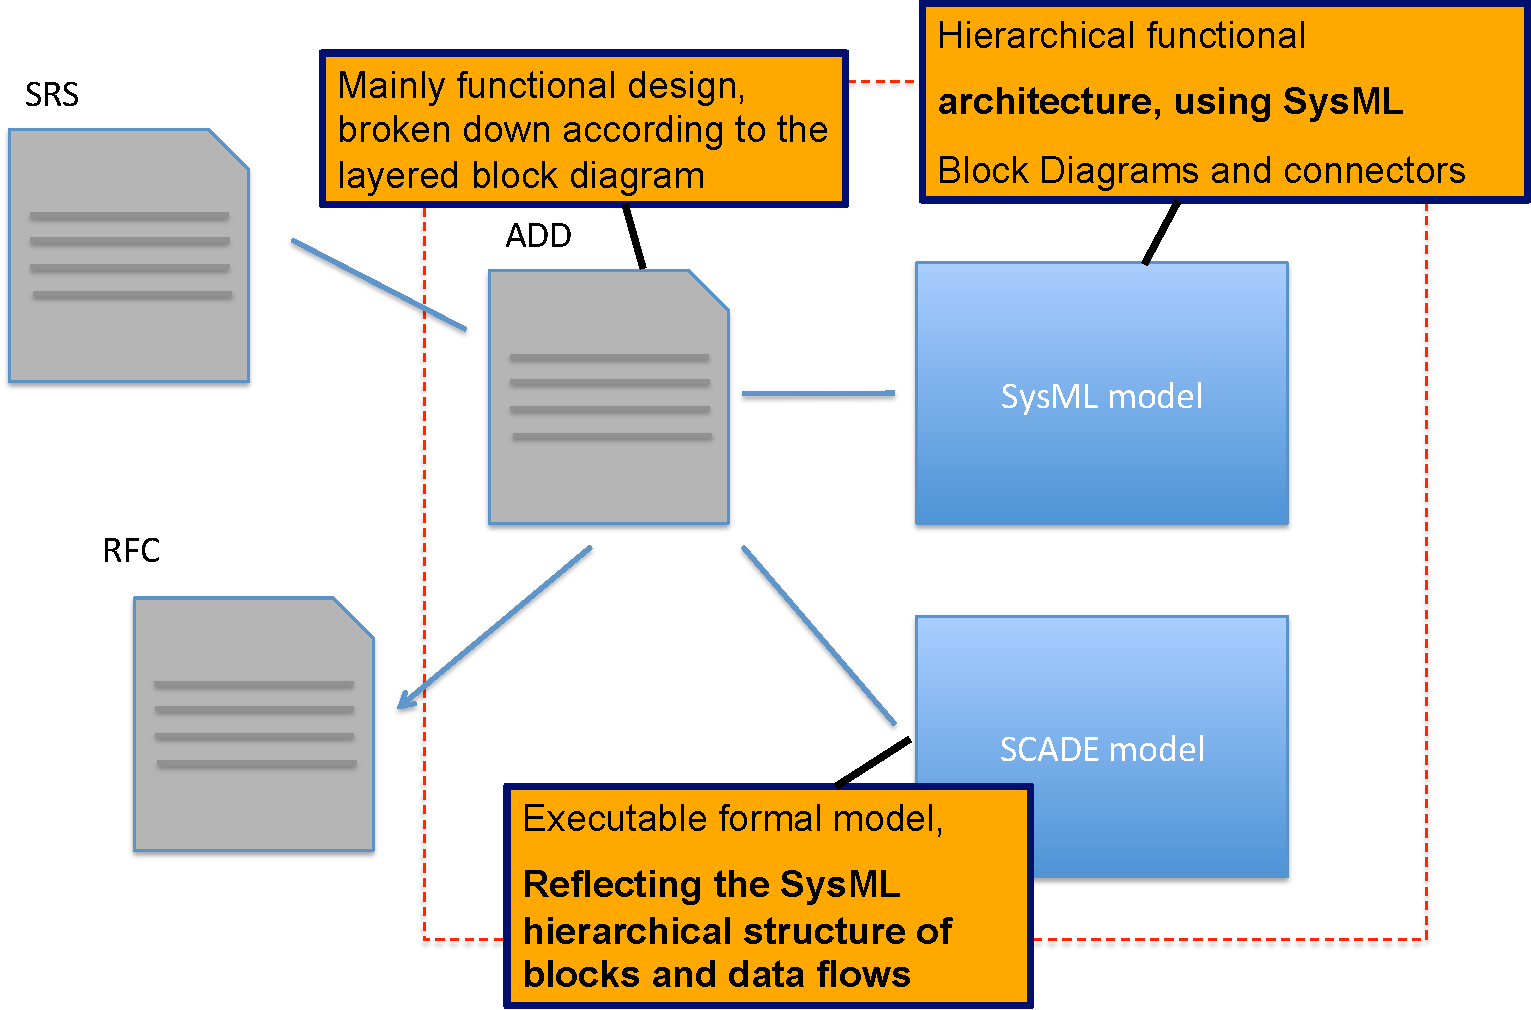
\includegraphics[width=\linewidth]{document-relations.pdf}
  \caption{Document relationships in WP3}
  \label{fig:doc-rels}
\end{figure}

Each main WP3 collateral has it's distinct role in the overall project structure. For a schematic view of the dependencies, see figure \ref{fig:doc-rels}. \\


\textbf{Objectives and scope related to the ADD document (this document)}\\

 



The ADD document is intended to provide the following main information:

• Internal guidance for the project: Provide authoritative guidance on process, responsibilties, process and workflow.\\
 
• Architectural design description: Provide complete information on the overall architecture of the openETCS kernel functions.\\

• Functional design description: Provide comprehensive information on the design of the system, which includes QoS aspects, interfaces, data types, algorithms and finally the full software design.\\
\\

The nature of the development process implies that this document will be a "living document", meaning that it will be constantly updated, with new iterations being planned as follows:

•  Intermediate work iterations (0.x): as required until the ITEA2 intermediate review (March 2015)

• First main release (1.0): as a deliverable for the ITEA2 intermediate review (March 2015)

• Intermediate work iterations (1.x): as required until the demonstrator milestone (June 2015)

•  Second main release (2.0): for the demonstrator milestone (June 2015)

•  Intermediate work iterations (2.x) for the rest of the project duration (until Oct 2015)

•  Final release (3.0) for the final review.

Intermediate work iteration shall be managed using the normal day-to-day pull/ review process, while main releases require a formal document sign-off.\\

\textbf{Objectives and scope related to User Validation Scenario Document}\\

The work of WP3 has now been aligned to the milestones that are relevant for the overall project:

•  (1) ITEA2 intermediate review (March 2015)

•  (2) Demonstrator milestone (June 2015)

•  (3) Final review (End of 2015)

In order to support the functional approach, we use operational scenarios that are described the the User Validation Scenario Document.

These are based on the following data:

•  Rules from NS for the operation of trains

•  Infrastructure data from the Utrecht- Amsterdam line

In order to support the functional analysis, which is aligned with the project's milestones, this document will define use cases along the following principles:

•  (1) Selected operational scenarios on selected sections of the Utrecht- Amsterdam track

Based on nominal scenarios, our simulated train will drive across actual (simulated) infrastructure, selecting only a few, typical balise groups.
This will allow WP3 to implement the relevant mode/level/message (balise and RBC) functionality first,

The openETCS kernel model has been complemented by a simple DMI representation, in order to validate actual behaviour. 

In march 2015, only basic scenarios will be demonstrated, which have been organised as use cases, based on a plant/ controller co-simulation concept.

The future 


•  (2) Selected operational scenarios on the full Utrecht- Amsterdam track

Based on nominal scenarios, our simulated train will drive across actual (simulated) infrastructure, covering the entire Utrecht- Amsterdam track.
This will allow WP3 to implement the relevant mode/level/message (balise and RBC) functionality first, fo full functional coverage of the test track.

Compared to the fist step in March, we will also cover more operational scenarios according to the NS operational rules.

A generic, interactive simulation concept will be created for this purpose. 

The entire track with its 488 balise groups and known (real) RBC messages as well as specific validation scenarios will be modelled.

A presentation of this concept can be found in the section "Dynamic Simulation".

•  (3) Full coverage of Utrecht- Amsterdam

For the final review, we will prepare a openETCS kernel software that can run defined scenarios, accordiing to the NS operation regulation, across the entire Utrecht- Amsterdam line, either replaying actual train rides or simulating various events, nominal and non- nominal.

In cooperation with WP4 and WP5 this will provide additional input for demonstration and validation.



\textbf{Objectives and scope related to the RFC process}\\


The RFC document is a deliverable that was added to the WP3 set of documents during the Nov 3-7, 2014 Munich workshop.\\

Most (industrial) ETCS OBU systems have been built based on pure SRS analysis. at least in theory. In practise, each implementation is derived from the SRS, but with a mindset that is partially driven by the company culture and local operational regulation prior to ERTMS introduction.\\
This has lead to a plethora of ETCS systems, which exhibit subtle differences which lead to incomplete compatibility between OBUs and track equipment of different suppliers. Each OBU works best on a track which was built by the same supplier in the same country.\\
One of the objectives of openETCS is to provide a reference design for an ETCS UBU that reduces these variations.\\
The experts of WP3 and WP4 agree that a functional approach will lead to a better understanding of the system. As the SRS remains the formal reference, we have to provide formal feedback which is traceable to the SRS.\\
This is the objective of the RFC document.

The RFC document shall be structured following the paragraphs in the SRS and shall provide full traceability to the openETCS ADD.
Each design decision that can be traced to a deviation from the SRS or that highlights inconsistencies inside the SRS shall be documented in the RFC.\\
The RFC is hence a deliverable that provides formal feedback to the relevant ERTMS stakeholders.\\

(we still have to discuss the precise interaction between the SRS Analysis effort, WP4 and this RFC document)

The nature of the development process implies that this document will be a "living document", meaning that it will be constantly updated, with new iterations being planned as follows:

•  Intermediate work iterations (0.x): as required until the ITEA2 intermediate review (March 2015)

• First main release (1.0): as a deliverable for the ITEA2 intermediate review (March 2015)

• Intermediate work iterations (1.x): as required until the demonstrator milestone (June 2015)

•  Second main release (2.0): for the demonstrator milestone (June 2015)

•  Intermediate work iterations (2.x) for the rest of the project duration (until Oct 2015)

•  Final release (3.0) for the final review.

Intermediate work iteration shall be managed using the normal day-to-day pull/ review process, while main releases require a formal document sign-off.\\


\textbf{Objectives and scope related to formal executable model}\\

During the previous iterations of this document, it was proposed to use a traditional waterfall model in order to define the architecture and subsequently the functional and software design of the openETCS kernel software.
We have now shifted the design paradigm to a more agile process, where we will use iterations (functional analysis, implementation of prototype formal executable model, refinement) in order to design the software modules. (bottom- up design of modules)\\
These will then be merged into a top- down architecture by the chief architect, using best practises that are well established for data- flow oriented software designs.\\

The result will be a functional, formal model, from which code can be generated that implements the functionality fo the various stages of the demonstrator, the final implementation on the Alstom EVC, the GE platform, and also additional platforms that may be contributed by the partners beyond the original scope of the project.\\



\section{Roles, responsibilities and tasks}
%\tbc
%Baseliyos Jacob
\textbf{In this section, the roles and responsibilities of the WP3 partners are confirmed, especially where they divert from what has been agreed upon at the start of WP3:}

\begin{itemize}
\item\textbf{Responsibilities} First of all, in the last WP 3 meeting in Brussels on  10.09.2014 DB proposed to take over the lead of the architecture design and functional breakdown. At the subsequent weekly scrum meeting on 12.09.2014,  it was agreed upon by all participants that DB will take over the lead (see Appendix … );\\
\item\textbf{Planning:} Alstom as WP 3 leader will remain to be responsible for the planning and the allocation of the defined tasks to the different partners\\
\item\textbf{Roles:} Alstom will also coordinate the work and safeguard that the defined results will be delivered according to the quality requirements that are agreed within the ITEA2 project and the schedule and the milestones that will be agreed upon during the coming workshops;\\
\item All WP3 partners will deliver the results or products according to planning as will be agreed upon during the said workshops. \\

In the interest of a swift production of the critical documentation of which this version is a draft, specific tasks will be defined in terms of concrete results to be delivered, the timeframes in which these results must be produced and the partner who shall be responsible for that specific result and the planning. This is to safeguard the timely delivery. The process will be described in the next sections.\\
\end{itemize}

\section{Concept and Process}


%\tbc
%JakobGärtner
%\begin{itemize}



\section{Assumptions and preconditions}
%\tbc
%Baseliyos Jacob
\begin{itemize}
\item All future contributions shall be fully aligned an compliant the finalized and approved document 
\item Alls documents produced by the partners are requested to be compliant and merge to this document; other contributions will be discarded
\textbf{The workshops are all about working as swift, as efficient and as productive as possible and make full use of the potential made available for these workshops by the partners. It is expected that the partners in the workshops will have the express intention to:}
\item Contribute to the workshops with the intention to finalize the openETCS architecture;\\
\item Provide resources according to the agreements made prior to the Workshops;\\
\item Focus primarily on  getting concrete results regardless of methodological issues that might arise. Where necessary or opportune, classical project management methodology will be applied;\\
\item Provide full transparency with respect to experience, knowledge base and information touching the subjects to be treated in the workshops;\\
\item Document on paper or electronically all output of the workshops and integrate these with the underlying document;\\
\item Restrict discussions only to topics that have an immediate impact on the content or the quality of the end product: the improved version of this document.\\
\end{itemize}

\section{openETCS history and iterations}
%\tbc
%BaseliyosJacob
The openETCS Architecture and Design wil implemented in iterations. The current step (third iteration) is based on a step to implement the kernel functions of the ETCS system. For a better understanding of the scope the Iteration is described in the following.

\textbf{Third Iteration Functional Scope: The OBU functions for Szenarios defined in chapter 3}

The openETCS third iteration architecture and the design of the openETCS OBU software as mainly specified in \cite{subset-026} UNISIG Subset\_026 version\_3.3.0. 

The appropriate functionality has been divided into a list of functions of different complexity to make it more managable by the different designer.

All these functions are object of the openETCS project and have to be analysed from their requirements and subsequently modelled and implemented. With the given manpower in WP 3, a reasonable selection and order of these functions is required for the practical work that allows the distribution of the workload, more openETCS participants to join and leads to an executable---limited---kernel function as soon as possible. 


\textbf{The first objective of this third iteration are:}
\begin{itemize}
\item ``Make the train run as soon as possible, on the scenarios defined in third iteration \textbf(see chapter 3), and in the form of a rapid prototype".
This does not contradict the openETCS goal to conform to EN50128.
\item After a phase of prototyping, the openETCS software shall be implemented in compliance to EN50128 for SIL4 systems.
\end{itemize}


=======
%-----------------------------------------------------------------------
%\subsection{Mode and Level}
%-----------------------------------------------------------------------
%\tbc
%

\section{Motivation}
%\tbc
%BaseliyosJacob
The openETCS work package 3 (WP3) aims to provide – amongst others - the software architecture for the openETCS kernel in order to eventually build the software itself. WP3  partner has put great effort in the openETCS software design, thus far without making definite choices on the software architecture itself respective of functional breakdown and data structures of the openETCS kernel. Since the project planning foresees in the production of a reference software to be used as a demonstrator by June 2015, it is of paramount importance that a first design delivarable of the openETCS kernel architecture be finalized shortly but no later than November 2014.\\

In compliance with the agreements made during the last WP 3 meeting at the 10.09.2014 in Brussels, DB has taken the initiative to design the aforesaid architecture including of functional breakdown and data structures in order to safeguard a timely delivery of these products. Furthermore, DB has ensured that these developments are focused on including end user requirements so as to develop a design in conformity with the needs and requirements of the operators. Specialists of DB and NS have cooperated together with other partners in WP3 to produce this document.\\

As referred to above, the architecture description has to be finalized in the month of November 2014. This version of the document is a draft version, demonstrating the general directions and philosophy of the architectural design, the functional breakdown of the software and the data structures. The design is focused on maximum efficiency in order to maximize on RAMS performance of the end product.\\


\section{Objectives}
%\tbc
%Baseliyos Jacob
The prime objective of WP3 is to produce a fully formal prototype for the openETCS reference system that can function as a demonstrator in collaboration with WP 4 and WP 5  for the openETCS approach and will be used as such in the final phase of the project. That phase is the first half of 2015.  This objective is defined as … 

\textbf{High level Objectives of this work:}
<<any further general statements on the ITEA2  objectives, like…>>\\

\begin{itemize}
\item Work on a model bases approach and process for effective collaborative work within an international ETCS developer team as stated above, the project needs a definite architecture design by the end of 2014.

\textbf{This document targets:}
\item Defining the general design and conditions of the openETCS architecture, functional breakdown and data structures
\item Providing the guidelines for discussion during the workshops that are planned in October and November 2014 that will result in the final and decisive version of this document
\item Being the ‘platform’ for finalization i.e. whatever be the products or results of the workshops shall be integrated in this document.

\textbf{Apart from these general objectives, the document means to provide for the materials that will enable WP3 partners to improve the efficiency of the Work Package activities:}
\item The comprehensive architecture design shall enable splitting the work load according to the building blocks defined by the architecture and allocate strictly compartmented work parcels or activities to WP3 partners.
\item Doing so will enable WP3 to avoid any double work
\item  Compartmenting the work load according to the functional building blocks as defined by the architecture will enable efficient planning of activities, be it individually or the integrated WP3 planning for the coming period, aiming at a just in time delivery of all results and products
\item  Compartment the work load according to the functional building blocks as defined by the architecture will enable efficient planning of activities, be it individually or the integrated WP3 planning for the coming period, aiming at a just in time delivery of all results and products
\end{itemize}

\section{Roles, responsibilities and tasks}
%\tbc
%Baseliyos Jacob
\textbf{In this section, the roles and responsibilities of the WP3 partners are confirmed, especially where they divert from what has been agreed upon at the start of WP3:}

\begin{itemize}
\item\textbf{Responsibilities} First of all, in the last WP 3 meeting in Brussels on  10.09.2014 DB proposed to take over the lead of the architecture design and functional breakdown. At the subsequent weekly scrum meeting on 12.09.2014,  it was agreed upon by all participants that DB will take over the lead (see Appendix … );\\
\item\textbf{Planning:} Alstom as WP 3 leader will remain to be responsible for the planning and the allocation of the defined tasks to the different partners\\
\item\textbf{Roles:} Alstom will also coordinate the work and safeguard that the defined results will be delivered according to the quality requirements that are agreed within the ITEA2 project and the schedule and the milestones that will be agreed upon during the coming workshops;\\
\item All WP3 partners will deliver the results or products according to planning as will be agreed upon during the said workshops. \\

In the interest of a swift production of the critical documentation of which this version is a draft, specific tasks will be defined in terms of concrete results to be delivered, the timeframes in which these results must be produced and the partner who shall be responsible for that specific result and the planning. This is to safeguard the timely delivery. The process will be described in the next sections.\\
\end{itemize}

\section{Process}
%\tbc
%JakobGärtner
\begin{itemize}
\item\textbf{Alstom as WP 3 leader will be responsible for planning}
\item\textbf{Time and quality aspects should be respected}
\item\textbf{openETCS tools and methodology must be respected}



\textbf{Most of the operational requirements to WP3 in the last phases of the ITEA2 project have been described in the former paragraphs. This section will describe the process which has to lead to the final result: the reference software to be used in the demonstrator next year, more specifically the final description of the openETCS architecture including the data structures and its functional decomposition. The process will run as follows:}

\item DB will supervise  the development of the first ‘firm’ draft of the specified products, ‘firm’ meaning that changes can only be made within the framework of these products and not to the fundamentals of these products as described in this document

\item DB will supervise the preparation of the two workshops that are proposed by Alstom and aim at defining the final and definite architecture, data structures and functional decomposition. It will make proposals for a planning of the critical tasks that remain to be done
\item Alstom will lead the two workshops following the preparations and the instructions of DB. Since all participants are intrinsically involved in the development work and tend to immerse themselves in technical discussions, for productivity purposes it is proposed to make use of a (non-technical) moderator that will be made responsible for coordinating the meeting, the discussions and the team efforts according ot the agenda.\\
\item Also for productivity reasons, introductory presentations will be restricted to the contents and setup of this document since all prior efforts have to be merged with this document and not the other way around. Following a general introduction into the work that has been so far, the other contributions will be scrutinized on their consistency with this document and any useful sections will be merged with this document.\\
\item During the workshops, there will be ample room reserved for enhancing this document, using other documents pertaining to the same field of work that have been delivered by other partners. Only material that is aligned with the general philosophy and structures proposed by this document, will be integrated;\\
\item In case conflicting views emerge over the benefits and value of certain contributions, at the very moment that parties conclude that they have conflicting views, these will be listed in an inventory for later discussion. The moderator shall note any such conflicts on the said inventory. Conflicting views will be treated at the end of each workshop whenever there is sufficient time or will be treated in a separate meeting that will be chaired by DB as coordinator of the ITEA2 project.\\
\item The workshop shall be attended by a secretary provided for by DB who is responsible for making the workshop minutes. Within a week after each workshop these minutes shall be distributed among the partners that have cooperated in the workshop and be reviewed by those. \\
\item The main objective of the workshops shall be the finalization of this document. In order to reach the specified result, the remaining tasks shall be identified and split into separate tasks or work parcels. Every task or work parcel will be allotted to one single responsible partner. Responsibility relates to the timely delivery of the defined result and according to quality requirements;\\
\item Alstom, as WP3 leader, will be responsible for the planning, allocation of tasks or work parcels to partners and will ensure timely delivery of results;\\
\item In case there will be tasks or work packages that cannot be finalized during the workshops or will be identified during the workshops and do not fit in the actual planning, these will be allotted in such a way that deadlines are perfectly clear and acknowledged by the party that is responsible for the results, fit within the general requirements of the project and are agreed upon in writing and executed by the responsible partners according to agreement;\\
\item DB as partner that has integral responsibility for both the ITEA2 project and responsible as well for the architecture etc. , is entitled to interfere take over the role as leader / coordinator in case the workshops prove to be insufficiently productive;\\
\item All output will be such, that it can be integrated in this document. It is the responsibility of DB to integrate the results and to deliver the final and definite version of this document. \\
\item The document concept will follow the openETCS process and tools (LaTex and Git-hub).\\

The figure below should demonstrate the process and workflow between the ERTMS and Modeling Experts within the openETCS Team.\\
\end{itemize}


\begin{figure}[h]
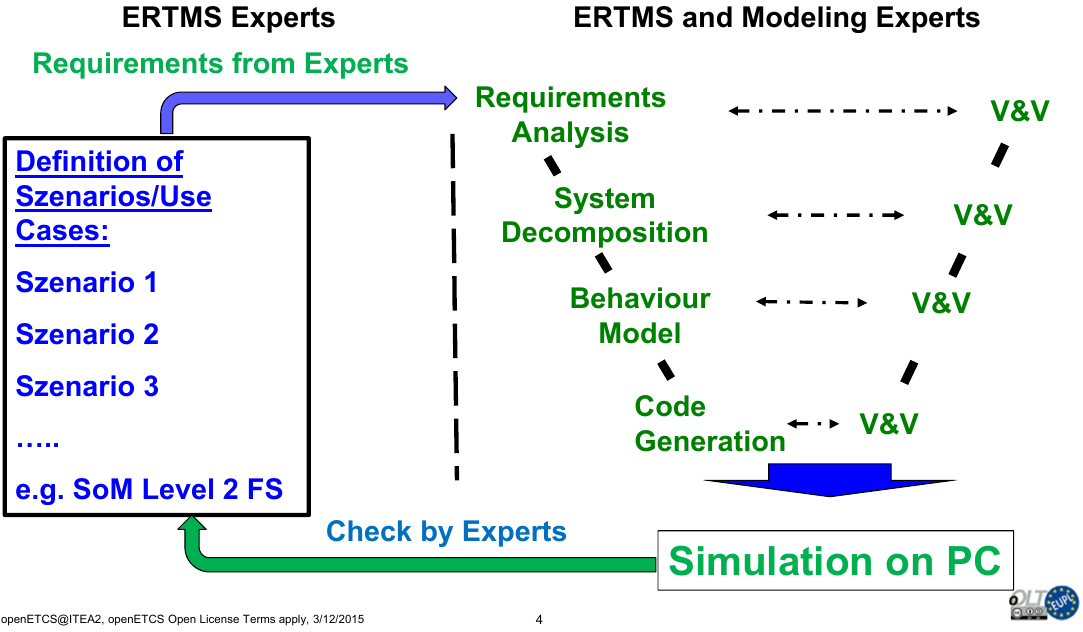
\includegraphics[scale=0.5]{images/Procedure}
\caption{Process within the openETCS Process}
\label{Process within the openETCS Process}
\end{figure}

\section{Assumptions and preconditions}
%\tbc
%Baseliyos Jacob
\begin{itemize}
\item All future contributions shall be fully aligned an compliant the finalized and approved document 
\item Alls documents produced by the partners are requested to be compliant and merge to this document; other contributions will be discarded
\textbf{The workshops are all about working as swift, as efficient and as productive as possible and make full use of the potential made available for these workshops by the partners. It is expected that the partners in the workshops will have the express intention to:}
\item Contribute to the workshops with the intention to finalize the openETCS architecture;\\
\item Provide resources according to the agreements made prior to the Workshops;\\
\item Focus primarily on  getting concrete results regardless of methodological issues that might arise. Where necessary or opportune, classical project management methodology will be applied;\\
\item Provide full transparency with respect to experience, knowledge base and information touching the subjects to be treated in the workshops;\\
\item Document on paper or electronically all output of the workshops and integrate these with the underlying document;\\
\item Restrict discussions only to topics that have an immediate impact on the content or the quality of the end product: the improved version of this document.\\
\end{itemize}

\section{openETCS history and iterations}
%\tbc
%BaseliyosJacob
The openETCS Architecture and Design willb de documented and implemented in iterations. 

\begin{itemize}
\item \textbf{first iteration can be downloaded under the following link:}
\end{itemize}


\begin{itemize}
\item \textbf{second iteration has not been published due some technical issues and will fully substituded by the third iteration.}
\end{itemize}

\begin{itemize}
\item \textbf{first iterationcan be downloaded under the following link:}
\end{itemize}
The current step (third iteration) is based on a step to implement the kernel functions of the ETCS system. For a better understanding of the scope the Iteration is described in the following.

\textbf{Third Iteration Functional Scope: The OBU functions for Szenarios defined in chapter 3}

The openETCS third iteration architecture and the design of the openETCS OBU software as mainly specified in \cite{subset-026} UNISIG Subset\_026 version\_3.3.0. 

The appropriate functionality has been divided into a list of functions of different complexity to make it more managable by the different designer.

All these functions are object of the openETCS project and have to be analysed from their requirements and subsequently modelled and implemented. With the given manpower in WP 3, a reasonable selection and order of these functions is required for the practical work that allows the distribution of the workload, more openETCS participants to join and leads to an executable---limited---kernel function as soon as possible. 


\textbf{The first objective of this third iteration are:}
\begin{itemize}
\item ``Make the train run as soon as possible, on the scenarios defined in third iteration \textbf(see chapter 3), and in the form of a rapid prototype".
This does not contradict the openETCS goal to conform to EN50128.
\item After a phase of prototyping, the openETCS software shall be implemented in compliance to EN50128 for SIL4 systems.
\end{itemize}


>>>>>>> ed68978492eb63cf6055ff353e29ef356af570a3
